\chapter{Scelte di progetto e cenni di teoria}\label{chap:scelte_di_progetto}

\section{Java Bean}\label{sec:java_bean}
Le JavaBean sono usate per incapsulare molti oggetti in un singolo oggetto (il bean), così da poter passare il bean invece degli oggetti individuali.
Al fine di funzionare come una classe JavaBean, una classe comune di un oggetto deve obbedire a certe convenzioni in merito ai nomi, alla costruzione e al comportamento dei metodi. 
Le convenzioni richieste sono:
\begin{itemize}
    \item La classe deve avere un costruttore senza argomenti.
    \item Le sue proprietà devono essere accessibili usando get, set e altri metodi (così detti metodi accessori).
    \item La classe dovrebbe essere serializzabile (capace di salvare e ripristinare il suo stato in modo persistente).
    \item Non dovrebbe contenere alcun metodo richiesto per la gestione degli eventi.
\end{itemize}

Utilizzando queste proprietà, i Java Bean sono risultati molto utili sia per creare strutture facilmente inviabili via rete, sia per utilizzare le classi XMLEncoder e XMLDecoder per scrivere e leggere Java Bean da file XML.

\section{UML Logica}\label{sec:UML_logica}
\begin{figure}[t]
 \centering
 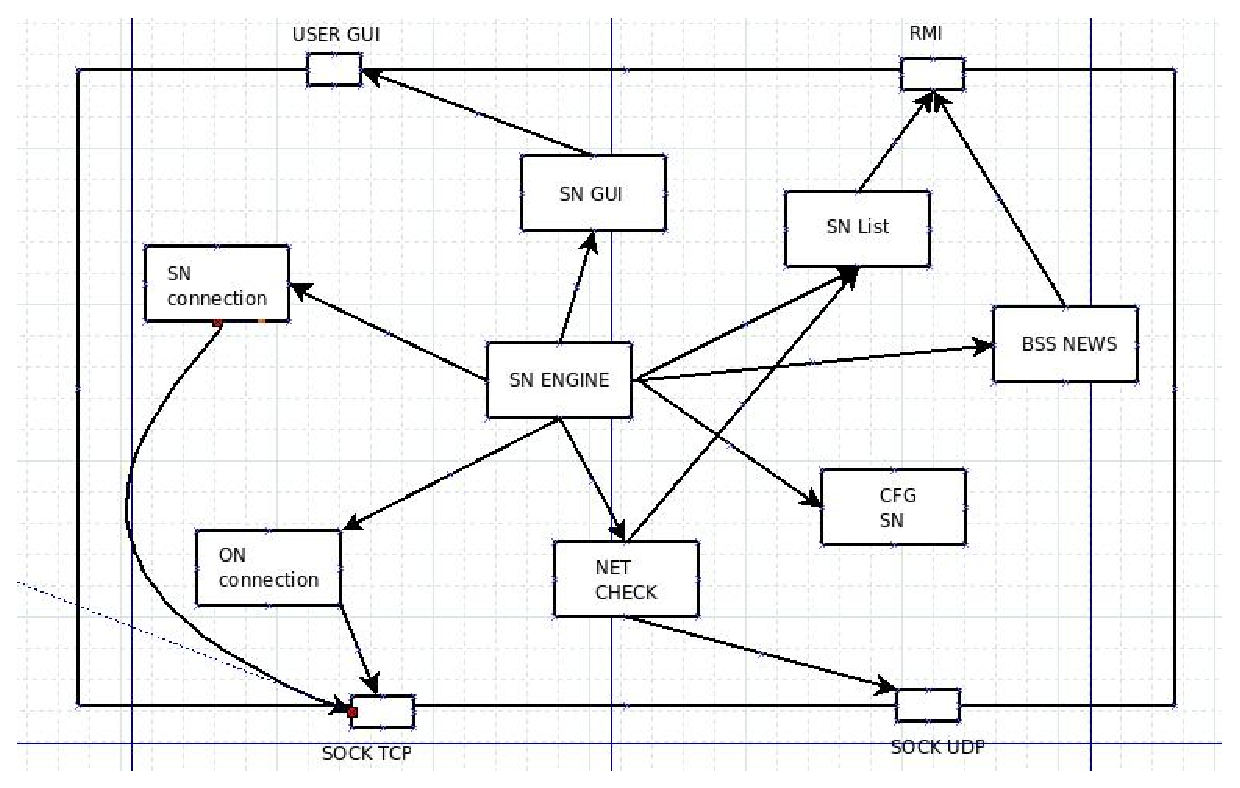
\includegraphics[width=400px,height=225px,bb=14 14 593 376]{images/logica_uml.eps}
 % logica_uml.eps: 0x0 pixel, 300dpi, 0.00x0.00 cm, bb=14 14 593 376
 \caption{Il diagramma UML che rappresenta la logica di Mini-KaZaA.}
 \label{fig:logica_uml}
\end{figure}
%Inserire una breve descrizione del diagramma UML
La logica del programma è visualizzabile in Figura \ref{fig:logica_uml}.
Il diagramma UML si riferisce un nodo di tipo SN, ma, visto che possiamo considerare i SN come degli ON con alcune funzionalità in più, questo diagramma vale anche per gli ON.

Possiamo vedere come ogni nodo abbia due tipi di componenti:
\begin{itemize}
 \item componenti logica interna;
 \item componenti di interfaccia con il mondo esterno.
\end{itemize}

Tutti questi componenti vengono gestiti da un motore centrale che richiama opportunamente le strutture dati utilizzate e i thread che devono svolgere i vari compiti.


\section{Classe Wrapper per il socket}\label{sec:wrap_sock}
Il fine del Wrapper è di fornire una soluzione astratta al problema dell'interoperabilità tra interfacce differenti. Il problema si presenta ogni qual volta nel progetto di un software si debbano utilizzare sistemi di supporto (come per esempio librerie) dotati di interfaccia non perfettamente compatibile con quelle richieste da applicazioni già esistenti. Invece di dover riscrivere parte del sistema, oneroso e non sempre possibile se non si ha a disposizione il codice sorgente, può essere comodo scrivere un Adapter che faccia da tramite tra le diverse interfacce, rendendole così compatibili.

Il wrapper inoltre ci ha consentito di poter inizializzare un oggetto che ci serviva all'interno di un \emph{sotto-thread} all'interno dell'\emph{engine} per poi modificarne il contenuto all'interno dei vari sotto-thread non appena si rendevano disponibili le informazioni per completarne la struttura.


\section{Il protocollo  TCP}
Il TCP nacque nel 1970 come frutto del lavoro di un gruppo di ricerca del dipartimento di difesa statunitense. I suoi punti di forza sono l'alta affidabilità e robustezza.
Il protocollo TCP serve a creare degli stream socket, cioè una forma di canale di comunicazione che stabilisce una connessione stabile fra due stazioni, in modo che queste possano scambiarsi dei dati.

Il servizio offerto da TCP è il trasporto di un flusso di byte bidirezionale tra due applicazioni in esecuzione su host differenti. Il protocollo permette alle due applicazioni di trasmettere contemporaneamente nelle due direzioni, quindi il servizio può essere considerato "Full Duplex" anche se non tutti i protocolli applicativi basati su TCP utilizzano questa possibilità.
Il flusso di byte viene frazionato in blocchi per la trasmissione dall'applicazione a TCP (che normalmente è implementato all'interno del sistema operativo), per la trasmissione all'interno di segmenti TCP, per la consegna all'applicazione che lo riceve, ma questa divisione in blocchi non è per forza la stessa nei diversi passaggi.
TCP è un protocollo orientato alla connessione, ovvero prima di poter trasmettere dati deve stabilire la comunicazione, negoziando una connessione tra mittente e destinatario, che viene esplicitamente chiusa quando non più necessaria. Esso quindi ha le funzionalità per creare, mantenere e chiudere una connessione.
TCP garantisce che i dati trasmessi, se giungono a destinazione, lo facciano in ordine e una volta sola. Questo è realizzato attraverso vari meccanismi di acknowledgment e di ritrasmissione su timeout.
TCP possiede funzionalità di controllo di flusso e di controllo della congestione sulla connessione, attraverso il meccanismo della finestra scorrevole. Questo permette di ottimizzare l'utilizzo della rete anche in caso di congestione.

\section{Il protocollo UDP}
A differenza del TCP, l'UDP è un protocollo di tipo connectionless, inoltre non gestisce il riordinamento dei pacchetti né la ritrasmissione di quelli persi, ed è perciò generalmente considerato di minore affidabilità. È in compenso molto rapido ed efficiente per le applicazioni "leggere" o time-sensitive. Ad esempio, è usato spesso per la trasmissione di informazioni audio o video. Dato che le applicazioni in tempo reale spesso richiedono un ritmo minimo di spedizione, non vogliono ritardare eccessivamente la trasmissione dei pacchetti e possono tollerare qualche perdita di dati, il modello di servizio TCP può non essere particolarmente adatto alle loro caratteristiche. L'UDP fornisce soltanto i servizi basilari del livello di trasporto, ovvero:
\begin{itemize}
    \item multiplazione delle connessioni, ottenuta attraverso il meccanismo delle porte
    \item verifica degli errori mediante una checksum, inserita in un campo dell'intestazione del pacchetto.
\end{itemize}
mentre TCP garantisce anche il trasferimento affidabile dei dati, il controllo di flusso e il controllo della congestione.
L'UDP non tiene nota dello stato della connessione, dunque ha rispetto al TCP informazioni in meno da memorizzare. Un server dedicato ad una particolare applicazione che scelga UDP come protocollo di trasporto può supportare molti più client attivi.

\section{Remote Method Invocation}
In informatica, e in particolare nel contesto del linguaggio di programmazione object-oriented Java, Remote Method Invocation (invocazione remota di metodi) o RMI è una tecnologia che consente a processi Java distribuiti di comunicare attraverso una rete. Questa tecnologia include una API (application programming interface) il cui scopo esplicito è quello di rendere trasparenti al programmatore quasi tutti i dettagli della comunicazione su rete. Essa consente infatti di invocare un metodo di un oggetto remoto (cioè appartenente a un diverso processo, potenzialmente su una diversa macchina) quasi come se tale oggetto fosse "locale" (ovvero appartenente allo stesso processo in cui viene eseguita l'invocazione). In questo senso, la tecnologia RMI può essere ricondotta, da un punto di vista concettuale, all'idea di chiamata di procedura remota riformulata per il paradigma object-oriented (in cui, appunto, le procedure sono sostituite da metodi).
L'utilizzo di un meccanismo di invocazione remota di metodi in un sistema object-oriented comporta notevoli vantaggi di omogeneità e simmetria nel progetto, poiché consente di modellare le interazioni fra processi distribuiti usando lo stesso strumento concettuale che si utilizza per rappresentare le interazioni fra i diversi oggetti di una applicazione, ovvero la chiamata di metodo. 

\section{Utilizzo dei ThreadPool}\label{sec:thread_pool}
In molte applicazioni vengono creati thread il cui stato è quasi sempre sospeso, in attesa che si verifichi un evento. Altri thread potrebbero entrare in uno stato di inattività ed essere attivati solo periodicamente alla ricerca di informazioni sullo stato di una modifica o di un aggiornamento. Il polling del thread consente di utilizzare i thread in modo più efficiente fornendo all'applicazione un pool di thread di lavoro gestiti dal sistema. Un unico thread consente di controllare lo stato di varie operazioni di attesa in coda nel pool di thread. Quando un'operazione di attesa viene completata, la funzione di callback corrispondente viene eseguita da un thread di lavoro contenuto nel pool di thread.

\section{Come funzionano le query}\label{sec:risposte_vuote}
Per aiutare a comprendere il meccanismo che stà dietro al nostro sistema di comunicazione per la ricerca di un file abbiamo creato una semplice vignetta che facilita il tutto.
\begin{figure}[t]
 \centering
 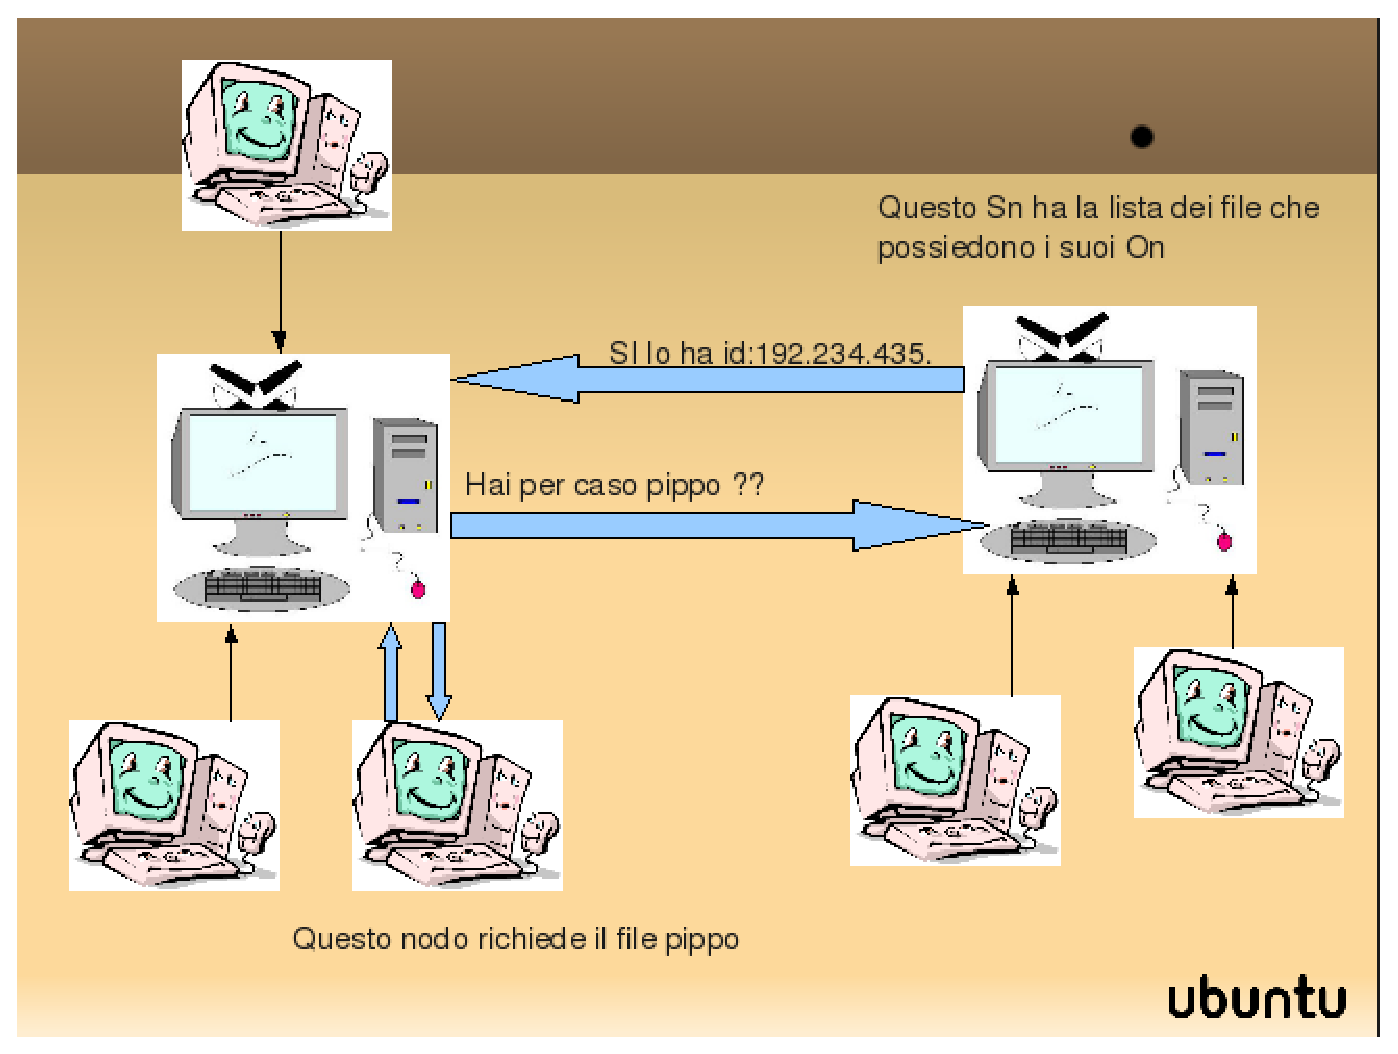
\includegraphics[width=300px,height=275px,bb=14 14 841 737]{images/pippo.eps}
 % mini_kazaa_client.eps: 0x0 pixel, 300dpi, 0.00x0.00 cm, bb=14 14 841 737
 \caption{Richiesta file.}
 \label{fig:richiesta_file}
\end{figure}
Ora che abbiamo trovato il file che desideriamo avviamo la comunicazione e lo scambio.
\begin{figure}[t]
 \centering
 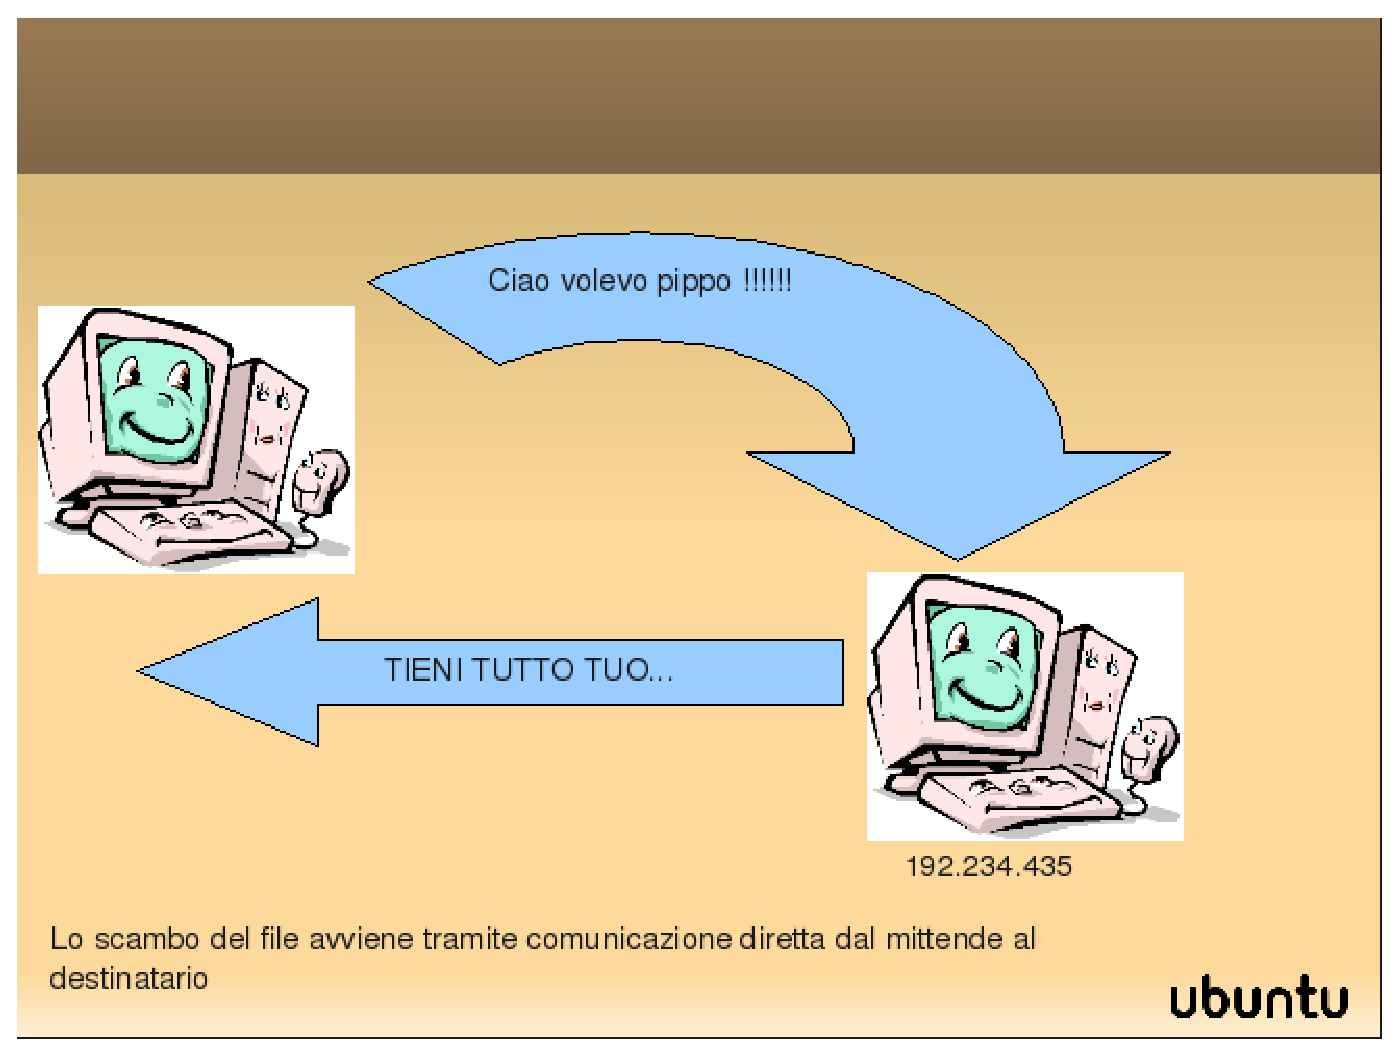
\includegraphics[width=300px,height=275px,bb=14 14 841 737]{images/pluto.eps}
 % mini_kazaa_client.eps: 0x0 pixel, 300dpi, 0.00x0.00 cm, bb=14 14 841 737
 \caption{Download.}
 \label{fig:download}
\end{figure}
%Spiegare perchè mandiamo risposte vuote.
